\section*{Appendix}
\subsubsection{Proof of \cref{cl:stlsound}.}
\begin{proof}
	Let $\varphi$ be an STL formula and $(S,{\hb})$ be a distributed signal.
	Assume $[(S,{\hb}) \models \varphi]_+ = \top$.
	We want to show that $[(S,{\hb}) \models \varphi] = \top$.
	Expanding the definition of $[(S,{\hb}) \models \varphi]_+ = \top$, we have $w \models \varphi$ for all $w \in \tr^+(S,{\hb})$.
	By \cref{cl:trsound}, we have $\tr(S,{\hb}) \subseteq \tr^+(S,{\hb})$.
	Then, it holds that $w \models \varphi$ for all $w \in \tr(S,{\hb})$.
	Therefore, $[(S,{\hb}) \models \varphi] = \top$ by definition.
	The case of $[(S,{\hb}) \models \varphi]_+ = \bot$ follows from the same arguments.
%	
%	\qed
\end{proof}

\subsubsection{Proof of \cref{cl:trsound}.}
\begin{proof}
	Let $(S,{\hb})$ be a distributed signal where $S = (x_1, \ldots, x_n)$.
	Let $w = (y_1, \ldots, y_n) \in \tr(S,{\hb})$ be a trace.
	We want to show that $w \in \tr^+(S,{\hb})$.
	First, let us recall the definition of $\tr^+$.
	\[ \tr^+(S,{\hb}) = \{ (x_1', \ldots, x_n') \st \text{$x_i'$ is consistent with $x_i$ for all $1 \leq i \leq n$}\} \]
	
	Let $1 \leq i \leq n$ be arbitrary.
	To show that $y_i$ is consistent with $x_i$, we need to show that $y_i$ is $I$-consistent with $x_i$ for all $I \in G_S$.
	Let $I = [t_0, s)$ be an arbitrary segment in $G_S$, let $(t_1, y_i(t_1)), \ldots, (t_\ell, y_i(t_\ell))$ be the edges of $y_i$ in segment $I$ with $t_j < t_{j+1}$ for all $1 \leq j < \ell$.
	To show that $y_i$ is $I$-consistent with $x_i$, we need to show that the expression $y_i(t_0) \cdot y_i(t_1) \cdot \ldots \cdot y_i(t_\ell)$ belongs to $\gamma(x_i,I)$.
	We sketch the proof idea below.
	
	Note that $w$ can be seen as a trace obtained through an $\varepsilon$-retiming of $S$ (\cite[Section 4.2]{MomtazAB23}).
	Then, the timestamp $t$ of any edge of $x_i$ is mapped to some clock value in the range $(\theta_{\text{lo}}(t), \theta_{\text{hi}}(t))$.
	In particular, $|t - c^{-1}_i(t)| < \varepsilon$ for all $t \in \{t_0, t_1, \ldots, t_\ell\}$, where $c^{-1}_i(t)$ is the local clock value of $x_i$ mapped to $t$.
	
	Since $y_i$ has $\ell$ edges in $I$, it holds that $x_i$ has at least $\ell$ edges in $(t_0 - \varepsilon, s + \varepsilon)$.
	Since $I$ is a segment in $G_S$, there are $\ell$ of these that are consecutive such that the intersection of their uncertainty regions contain $(t_0,s)$, i.e., $(t_0,s) \subseteq \bigcap_{1 \leq j \leq \ell} (\theta_{\text{lo}}(t_j'), \theta_{\text{hi}}(t_j'))$ where $t_j' = c^{-1}_i(t_j)$ is the corresponding timestamp in $x_i$ for all $0 \leq j \leq \ell$.
	In particular, note that $y_i(t_j) = x_i(t_j')$ for all $0 \leq j \leq \ell$.
		
	Now, notice that, by definition, $\gamma(x_i, I)$ takes into account every edge of $x_i$ whose uncertainty region has a nonempty intersection with $I$, and preserves their order.
	Let $V_j$ be the set of value expressions capturing how $I$ relates with the uncertainty intervals of the edge $(t_j', x_i(t_j'))$ for all $1 \leq j \leq \ell$ (as defined in \cref{eq:valexprset}).
	Then, $\destutter(\{x_i(t_0')\} \cdot V_1 \cdot \ldots \cdot V_\ell) \subseteq \gamma(x_i, I)$.
	One can verify that for all $1 \leq j \leq \ell$, either $x_i(t_j')$ or $x_i(t_{j-1}') \cdot x_i(t_j')$ belongs to $V_j$.
	This allows us to choose a value expression $v_j$ from each $V_j$ such that $\destutter(\{x_i(t_0')\} \cdot v_1 \cdot \ldots \cdot v_\ell) = x_i(t_0') \cdot x_i(t_1') \cdot \ldots \cdot x_i(t_\ell')$, which concludes the proof. 

	Note that if there are more edges of $x_i$ with a timestamp smaller than $t_0'$ or larger than $t_\ell'$ whose uncertainty intervals intersect with $I$, then the corresponding set of value expressions is obtained either by prefixing or suffixing.
	In either case, we can choose $\epsilon$ from these sets for concatenation with the remaining edges' value expressions and obtain the desired result.
%	
%	\qed
\end{proof}

\subsubsection{Proof of \cref{cl:algo}.}

We first introduce some notation and prove a technical lemma.
Then, we move on to prove \cref{cl:algo}. 

Let $x$ be a signal and $E_x = \{t_1, \ldots, t_m\}$ be the set of timestamps for its edges with $t_j < t_{j+1}$ for all $1 \leq j < m$.
We define the value expression $\pi(x) = x(0) \cdot x(t_1) \cdot \ldots \cdot x(t_m)$ encoding its initial value and edges.
Given a set $S$ of signals, we further define $\pi(S) = \{ \destutter(\pi(x)) \st x \in S \}$.

Let $w$ be a (synchronous) trace over a temporal domain $[0,d)$, and let $\varphi$ be an STL formula,
We define $y_{\varphi,w} : [0,d) \to \B$ as the satisfaction signal of $\varphi$ on input $w$.
Let $I = [s, s') \subseteq [0,d)$ be an interval.
We define $y_{\varphi,w,I} : [0, s' - s) \to \B$ as the slice of $y_{\varphi,w}$ over the interval $I$, i.e, $y_{\varphi,w,I}(t) = y_{\varphi,w}(t + s)$ for all $t \in [0, s' - s)$.
Given a set  $R$ of (synchronous) traces, we further define $Y(\varphi, R, I) = \{ y_{\varphi,w,I} \st w \in R \}$.

\begin{lemma} \label{cl:eq}
	Consider a distributed signal $(S,{\hb})$ with the canonical segmentation $G_S$ and an STL formula $\varphi$.
	For every segment $I \in G_S$ the following holds:
	\[ \pi(Y(\varphi, \tr^+(S,{\hb}), I)) = \llbracket (S,{\hb}), I \models \varphi \rrbracket \]
\end{lemma}
\begin{proof}
	The proof goes by induction on the structure of $\varphi$.
	Let $(S,{\hb})$ be a distributed signal, $\varphi$ an STL formula, and $I \in G_S$ a segment.
	We sketch each case below.
	
%	\vspace{1em}
	\noindent\textbf{Atomic propositions.}
	For the base case, let $\varphi = p$ for some $p \in \AP$.
	Note that $\llbracket (S, {\hb}), I \models p \rrbracket = \gamma(x_p, I)$ where $x_p$ is the signal encoding $p$.
	Moreover, by the definition of $\tr^+(S,{\hb})$, the set $Y(p, \tr^+(S,{\hb}), I)$ contains exactly the signals that are consistent with $x_p$ sliced over $I$.
	Then, it is easy to see that the set $\pi(Y(p, \tr^+(S,{\hb}), I))$ of value expressions coincide with $\gamma(x_p, I)$.
	
%	\vspace{1em}
	\noindent\textbf{Negation.}
	Let $\varphi = \lnot \psi$ for some formula $\psi$ such that $\pi(Y(\psi, \tr^+(S,{\hb}), I)) = \llbracket (S,{\hb}), I \models \psi \rrbracket$.
	Note that $\llbracket (S,{\hb}), I \models \lnot \psi \rrbracket$ contains exactly the bitwise negations of the Boolean value expressions in $\llbracket (S,{\hb}), I \models \psi \rrbracket$.
	Moreover, $Y(\lnot\psi, \tr^+(S,{\hb}), I)$ contains exactly the negation of the satisfaction signals in $Y(\psi, \tr^+(S,{\hb}), I)$.
	Then, clearly, $\pi(Y(\lnot\psi, \tr^+(S,{\hb}), I))$ contains exactly the bitwise negations of the expressions in $\pi(Y(\psi, \tr^+(S,{\hb}), I))$.
	Finally, since $\pi(Y(\psi, \tr^+(S,{\hb}), I)) = \llbracket (S,{\hb}), I \models \psi \rrbracket$, we obtain $\pi(Y(\lnot\psi, \tr^+(S,{\hb}), I)) = \llbracket (S,{\hb}), I \models \lnot\psi \rrbracket$.
	
%	\vspace{1em}
	\noindent\textbf{Conjunction.}
	Let $\varphi = \psi_1 \land \psi_2$ for some formulas $\psi_1, \psi_2$ such that $\pi(Y(\psi_i, \tr^+(S,{\hb}), I)) = \llbracket (S,{\hb}), I \models \psi_i \rrbracket$ for each $i \in \{1,2\}$.
	Note that $\llbracket (S,{\hb}), I \models \psi_1 \land \psi_2 \rrbracket$ contains exactly the bitwise conjunction of the pairs of value expressions in the asynchronous product of $\llbracket (S,{\hb}), I \models \psi_1 \rrbracket$ and $\llbracket (S,{\hb}), I \models \psi_2 \rrbracket$, or equivalently those of $\pi(Y(\psi_1, \tr^+(S,{\hb}), I))$ and $\pi(Y(\psi_2, \tr^+(S,{\hb}), I))$ by our initial assumption.
	Since the formulas are copyless and the signals are completely asynchronous within $I$, this set equals $\pi(Y(\psi_1 \land \psi_2, \tr^+(S,{\hb}), I)))$.
	
	More formally, consider the following:
	For each $u \in \destutter(\{ u_1 \BitAnd u_2 \st (u_1,u_2) \in \pi(Y(\psi_1, \tr^+(S,{\hb}), I)) \otimes \pi(Y(\psi_2, \tr^+(S,{\hb}), I))\})$, there exist two satisfaction signals $y_1 \in Y(\psi_1, \tr^+(S,{\hb}), I)$ and $y_2 \in Y(\psi_2, \tr^+(S,{\hb}), I)$ such that bitwise conjunction of $\pi(y_1)$ and $\pi(y_2)$ gives us $u$ -- this follows from the definition.
	Because the formulas are copyless and the signals are completely asynchronous within $I$, there exists a signal $y \in Y(\psi_1 \land \psi_2, \tr^+(S,{\hb}), I)$ that is exactly the conjunction of $y_1$ and $y_2$.
	Moreover, $\pi(y) = u$.
	
	Conversely, consider a value expression $u \in \pi(Y(\psi_1 \land \psi_2, \tr^+(S,{\hb}), I)))$ and let $y \in Y(\psi_1 \land \psi_2, \tr^+(S,{\hb}), I)$ be the signal with $\pi(y) = u$.
	Consider the corresponding trace $w \in \tr^+(S,{\hb})$ with $y = y_{\psi_1 \land \psi_2, w, I}$.
	Clearly, we have $y_{\psi_1, w, I} \in Y(\psi_1, \tr^+(S,{\hb}), I)$ and $y_{\psi_2, w, I} \in Y(\psi_2, \tr^+(S,{\hb}), I)$.
	Let $(u_1,u_2)$ be a pair of value expressions of the same length obtained from $y_{\psi_1, w, I}$ and $y_{\psi_2, w, I}$ by sampling both signals at time 0 and whenever one of the signals has an edge.
	It is easy to see that $(u_1,u_2)$ belongs to $\pi(Y(\psi_1, \tr^+(S,{\hb}), I)) \otimes \pi(Y(\psi_2, \tr^+(S,{\hb}), I))$.
	
%	\vspace{1em}
	\noindent\textbf{Untimed until.}
	Let $\varphi = \psi_1 \until \psi_2$ for some formulas $\psi_1, \psi_2$ such that $\pi(Y(\psi_i, \tr^+(S,{\hb}), I)) = \llbracket (S,{\hb}), I \models \psi_i \rrbracket$ for each $i \in \{1,2\}$.
	The key difference to the case of conjunction is that this is a temporal operator whose values at segment $I$ depends on the future segments.
	
	Let $G_S = \{ I_1, \ldots, I_m, I, J_1, \ldots J_k \}$ be the canonical segmentation where the segments are given in an increasing order of their left end points.
	Let us consider the last segment $J_k \in G_S$.
	By hypothesis, $\pi(Y(\psi_i, \tr^+(S,{\hb}), J_k)) = \llbracket (S,{\hb}), J_k \models \psi_i \rrbracket$ for each $i \in \{1,2\}$.
	By the same arguments as for conjunction, we have $\pi(Y(\psi_1 \until \psi_2, \tr^+(S,{\hb}), J_k)) = \llbracket (S,{\hb}), J_k \models \psi_1 \until \psi_2 \rrbracket$.
	Now, let us consider the segment $J_{k-1}$.
	We need to take into account whether $\psi_1 \until \psi_2$ is satisfied at the beginning of $J_k$.
	When it is satisfied (resp. violated), we can treat the undefined value of $\psi_1 \until \psi_2$ at the end of $J_{k-1}$ as true (resp. false).
	Note that these respectively correspond to weak until and strong until.
	Then, one can verify using the definitions that $\pi(Y(\psi_1 \until \psi_2, \tr^+(S,{\hb}), J_{k-1})) = \llbracket (S,{\hb}), J_{k-1} \models \psi_1 \until \psi_2 \rrbracket$.
	Repeating this down to segment $I$, we obtain the desired outcome.
	
%	\vspace{1em}
	\noindent\textbf{Timed until.}
	Let $\varphi = \psi_1 \until_J \psi_2$ for some interval $J$ and formulas $\psi_1, \psi_2$ such that $\pi(Y(\psi_i, \tr^+(S,{\hb}), I)) = \llbracket (S,{\hb}), I \models \psi_i \rrbracket$ for each $i \in \{1,2\}$.
	The key difference to the case of untimed until is that we need to take into account the profiles of $J$ with respect to $(S,{\hb})$, $\psi_1$, $\psi_2$, and $I$.
	
	We want to show that $\pi(Y(\psi_1 \until_J \psi_2, \tr^+(S,{\hb}), I)) = \llbracket (S,{\hb}), I \models \psi_1 \until \psi_2 \rrbracket$.
	First, recall that $\llbracket (S,{\hb}), I \models \psi_1 \until_J \psi_2 \rrbracket = \destutter( \{ u_1 \mathsf{U}^0 u_2 \st (u_1, u_2) \in P^1_1 \otimes P^2_1 \} \cdot \ldots \cdot \{ u_1 \mathsf{U}^0 u_2 \st (u_1, u_2) \in P^1_k \otimes P^2_k \} )$ where, for each $i \in \{1,2\}$, we have $\mathsf{pfs}((S,{\hb}), \psi_i, I, J) = \{P^i_1, \ldots, P^i_k\}$.
	Here, $P^i_j = \mathsf{profile}((S,{\hb}), \psi_i, I, J_j)$ for each $1 \leq j \leq k$ where $J_j$ is a representative among (potentially infinitely many) intervals with the same profile.
	Note that $\mathsf{pfs}$ and $\mathsf{profile}$ considered each $J_j$ as well as $J$ relative to $I$.
	To talk about these intervals without a reference point as $I$, we let $K_j = I \oplus J_j$ for each $1 \leq j \leq k$.
	We claim that $\mathsf{profile}((S,{\hb}), \psi_i, I, J_j) = \pi(Y(\psi_1, \tr^+(S,{\hb}), K_j))$ for each $1 \leq j \leq k$.
	This holds by hypothesis and the definition of $\tr^+$.
	
	Given an interval $K$, let use define $\tr^+_K(S,{\hb})$ as the projection of the traces in $\tr^+(S,{\hb})$ to the interval $K$.
	Then, we have $\llbracket (S,{\hb}), I \models \psi_1 \until_J \psi_2 \rrbracket = \destutter( \pi(Y(\psi_1 \until \psi_2, \tr^+_{K_1}(S,{\hb}), K_1)) \cdot \ldots \cdot \pi(Y(\psi_1 \until \psi_2, \tr^+_{K_k}(S,{\hb}), K_k)) )$.
	Now, we argue below that the left-hand side equals $\pi(Y(\psi_1 \until_J \psi_2, \tr^+(S,{\hb}), I ))$, concluding the proof.

	Let $y_j \in Y(\psi_1 \until \psi_2, \tr^+_{K_j}(S,{\hb}), K_j)$ for each $1 \leq j \leq k$.
	Then, using the arguments of copylessness and asynchronicity within segments as before, we can show that there exists $y \in Y(\psi_1 \until_J \psi_2, \tr^+(S,{\hb}), I)$ such that $\pi(y) = \destutter( \pi(y_1) \cdot \ldots \cdot \pi(y_k) )$.
	The other direction can be proved using the hypothesis and the definition of $\tr^+$.
%	
%	\qed
\end{proof}

We now proceed to prove \cref{cl:algo}.

\begin{proof}[of \cref{cl:algo}]
	Consider a distributed signal $(S,{\hb})$ and an STL formula $\varphi$.
	Assume $[(S,{\hb}) \models \varphi]_+ = \top$.
	It means that for every trace $w \in \tr^+(S,{\hb})$, the corresponding satisfaction signal's initial value is 1, i.e., $y_{\varphi,w}(0) = 1$.
	By \cref{cl:eq}, this also holds for $\llbracket (S, {\hb}) \models \varphi \rrbracket$.
	Now, assume  $\llbracket (S, {\hb}) \models \varphi \rrbracket = \{1\}$.
	It means that every value expression encoding the satisfaction of $\varphi$ (computed through recursive applications of the semantics function) start with 1.
	By \cref{cl:eq}, this also holds for $\pi(Y(\varphi, \tr^+(S,{\hb}), I))$ where $I$ is the first segment in $G_S$.
	Then, for all $y \in Y(\varphi, \tr^+(S,{\hb}), I)$ we have $y(0) = 1$, which means every $w \in \tr^+(S,{\hb})$ satisfies $\varphi$, and thus $[(S,{\hb}) \models \varphi]_+ = \top$.
	The cases of $\bot$ and ${\,?}$ are similar.
%
%	\qed
\end{proof}


\subsection*{ADD THESE TO SECTION 6}

\begin{figure}[htb]
	\begin{center}
		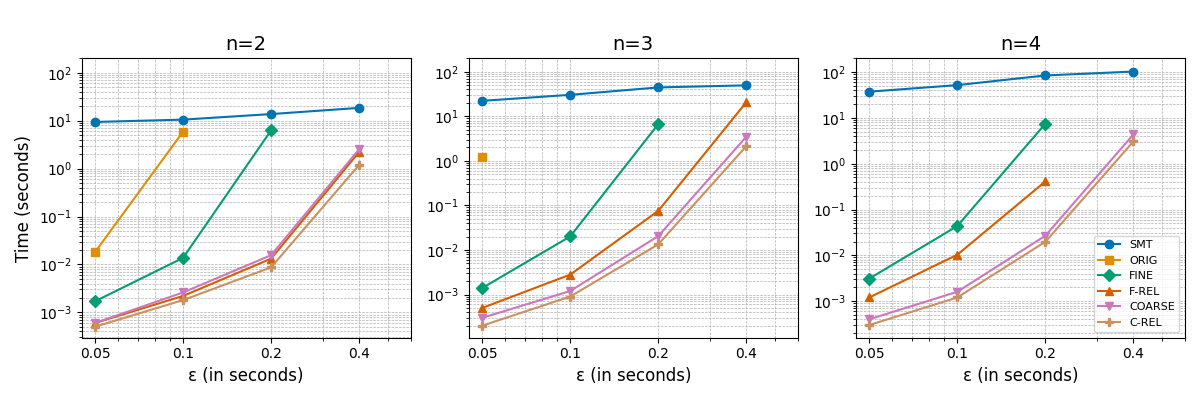
\includegraphics[width=\linewidth]{wt.png}
		\caption{Water tanks}
	\end{center}
\end{figure}

\subsubsection{Water Tanks Discussion.}
\TODO

\begin{figure}[htb]
	\begin{center}
		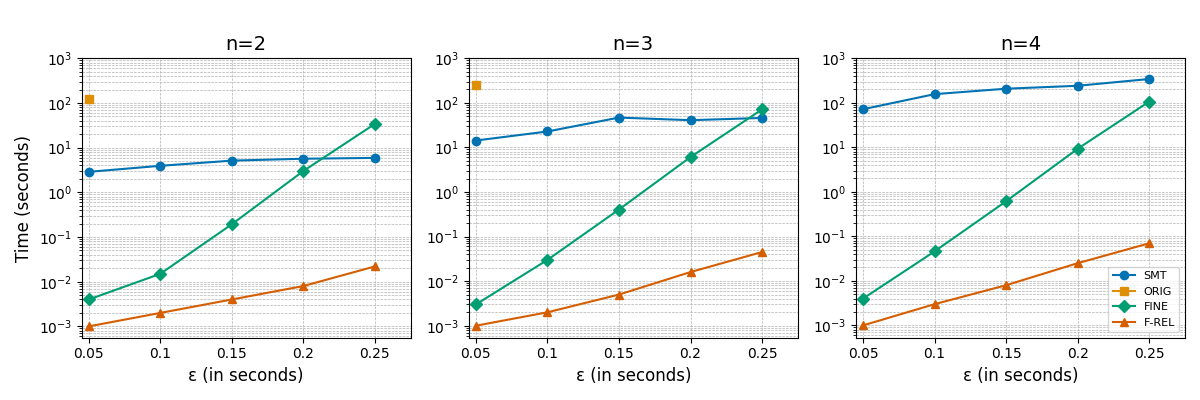
\includegraphics[width=\linewidth]{ms.png}
		\caption{Mutual separation}
	\end{center}
\end{figure}

\subsubsection{Mutual Separation Discussion.}
\TODO